% ======================================================================


% Sujet du document
% Informations importantes
%
%
% Prénom Nom
% H. Dube 2019
% ======================================================================
% Ce code rassemble les efforts d'étudiants de la faculté de génie  
% de l'université de Sherbrooke afin de faire un template LaTeX moderne
% dédié à l'écriture de rapport universitaire.
% Ce document est libre d'être utilisé et modifié.
% ======================================================================

% ----------------------------------------------------
% Initialisation
% ----------------------------------------------------
\documentclass{udes_rapport} % Voir udes_rapport.cls

\begin{document}
\selectlanguage{french}

% ----------------------------------------------------
% Configurer la page titre
% ----------------------------------------------------

% Information
\faculte{Génie}
\departement{génie électrique et génie informatique}
\app{3}{Modélisation et identification de systèmes dynamiques}
\professeur{Jean-Baptiste Michaud}
\etudiants{Hubert Dubé - dubh3401 \\ Gabriel Lavoie - lavg2007}
\dateRemise{2 octobre 2019}


% ======================================================================
\pagenumbering{roman} % met les numéros de pages en romain
% ----------------------------------------------------
% Page titre
% ----------------------------------------------------
\fairePageTitre{LOGO} % Options: [STD, LOGO]
\newpage

% ----------------------------------------------------
% Table des matières
% ----------------------------------------------------
\tableofcontents
\newpage


% ----------------------------------------------------
% Table des figures
% ----------------------------------------------------
\listoffigures
\newpage



% ======================================================================
% Document
% ======================================================================
\pagenumbering{arabic} % met des chiffres arabes
\setcounter{page}{1} % reset les numéros de pages
%%%%%%%%%%%%%%%%%%%%%%%%%%%%%%%%%%%%%%%%%%%%%%%%%%%%%%
%{Analyse du signal
%%%%%%%%%%%%%%%%%%%%%%%%%%%%%%%%%%%%%%%%%%%%%%%%%%%%%%
\section{Introduction}
La compagnie EstampBeauce a donné le mandat à notre équipe de modéliser un système permettant d'asservir la 
position angulaire d'une antenne. Les trois systèmes, soit électrique, électromécanique et mécanique, sont décrits séparément. 
Par la suite, une analyse complète du mécanisme est fournie en représentation d'état et par sa fonction de transfert.

\section{Équations physiques du système}
\subsection{Système électrique}
Le système électrique sert à transformer le signal d'entrée $e_in$ en tension $e_in$ qui alimente le moteur.
Il s'agit d'un amplificateur avec une réponse correspondant à un système d'ordre 1, dont l'équation est la suivante.

\begin{equation}
\frac{de_a}{dt} = \frac{K}{\tau}e_{in} - \frac{1}{\tau}e_a
\end{equation}

\subsection{Système électromécanique}
Le moteur à courant continu permet de convertir l'énergie électrique en rotation. 
L'analyse de la dynamique du système donne l'équation suivante.
\begin{equation}
\frac{di_a}{dt} = \frac{1}{L_a}e_a-\frac{R_a}{L_a}i_a - \frac{1}{L_a}e_b
\end{equation}

La force contre-électromotrice de moteur est définie en fonction de sa vitesse angulaire par l'équation suivante.
\begin{equation}
e_b = K_b\omega_m
\end{equation}

En insérant (3) dans (2), on obtiens l'équation différentielle du courant $i_a$
\begin{equation}
\frac{di_a}{dt} = \frac{1}{L_a}e_a-\frac{R_a}{L_a}i_a - \frac{K_b}{L_a}\omega_m
\end{equation}

\subsection{Système mécanique}
On considère ici que l'arbre reliant la transmission et la charge est rigide.
L'équation dynamique du système mécanique est la suivante.
\begin{equation}
J_m\frac{d\omega_m}{dt} = T_m - T_l - B_m\omega_m
\end{equation}
Le couple du moteur est défini en fonction du courant d'armature
\begin{equation}
T_m = K_ii_a
\end{equation}
Le couple de la charge est simplement défini par sa friction et son inertie. On transforme ensuite cette équation pour obtenir le couple de la charge 
tel que vu du côté du moteur.
\begin{equation}
T_l = \frac{d\omega_l}{dt}J_l + B_l\omega_l = N^2\frac{d\omega_m}{dt}J_l + N^2B_l\omega_m
\end{equation} 
Insérer (6) et (7) dans (5) donne une expression pour la vitesse angulaire du moteur.
\[ \frac{d\omega_m}{dt} = \frac{K_ii_a}{N^2J_l + J_m} - \frac{N^2B_l + B_m}{N^2J_l + J_m}\omega_m \]
Finalement, on transforme l'équation en utilisant $\omega_m = \omega_l/N$ pour obtenir la forme désirée.
\begin{equation}
\frac{d\omega_l}{dt} = \frac{NK_ii_a}{N^2J_l + J_m} - \frac{N^2B_l + B_m}{N^2J_l + J_m}\omega_m
\end{equation} 

\section{Variables et équations d'état}
Les quatre variables d'état du système sont $\theta_l$, $\omega_l$, $i_a$ et $e_a$.
On utilise les équations (1), (4) et (8), ainsi que la suivante, pour décrire le système.
\begin{equation}
\frac{d\theta_l}{dt} = \omega_l
\end{equation}
On obtiens donc la représentation d'état en forme ABCD.
\
$$
\begin{bmatrix}
\dot{\theta_l} \\
\dot{\omega_l} \\
\dot{i_a} \\
\dot{e_a} 
\end{bmatrix}
=
\begin{bmatrix}
0 & 1 & 0 & 0 \\
0 & \frac{-(N^2B_l + B_m)}{N^2J_l + J_m} & \frac{NK_i}{N^2J_l + J_m} & 0 \\
0 & \frac{K_b}{NL_a} & \frac{-R_a}{L_a} & \frac{1}{L_a} \\
0 & 0 & 0 & \frac{-1}{\tau}
\end{bmatrix}
\begin{bmatrix}
\theta_l \\
\omega_l \\
i_a \\
e_a 
\end{bmatrix}
+
\begin{bmatrix}
0 \\
0\\
0\\
\frac{K}{\tau}
\end{bmatrix} 
e_{in}
$$

$$
y(t) = 
\begin{bmatrix}
1 & 0 & 0 & 0
\end{bmatrix} 
\begin{bmatrix}
\theta_l \\ \omega_l \\ i_a \\ e_a
\end{bmatrix} 
$$


\subsection{Représentation graphique}
Sous forme de schéma bloc, le système peut être représenté à la figure \ref{fig:bloc}.
\insertFigure{open_closed_loop}{0.7}{Schéma bloc du système}{fig:bloc}
La partie en noire correspond au circuit en boucle ouverte et avec l'ajout de la partie en rouge, il s'agit du circuit en boucle fermé. Le même schéma peut être obtenu sous forme de graphe de fluence à la figure \ref{fig:fluence}.
\insertFigure{graphe_fluence}{0.7}{Graphe de fluence du système}{fig:fluence}
Encore une fois, la boucle ouverte est en noir et la boucle fermée est en rouge. Dans les deux figures, les fonctions $G$ représentent les fonctions d'ordre 1 déclarées au début de cette section.
\subsection{Représentation en fonction de transfert}
Afin d'obtenir la fonction de transfert en boucle ouverte (FTBO) la loi de Masson est appliqué sur la partie noire de la figure \ref{fig:bloc}. De manière analytique, la FTBO peut être représentée comme :
\begin{equation}
M = \frac{\theta_L}{e_{in}} = \frac{G_0 G_1 G_2 G_4}{1 + G_1 G_2 G_3}
\label{eq:FTBO}
\end{equation}
Comme les paramètres de la FTBO sont connues, elle peut être exprimée par :
\begin{equation}
M = \frac{\theta_L}{e_{in}} = \frac{2.083e06}{s^4 + 1101s^3 + 1.018e05s^2 + 1.708e05s}
\label{eq:nmum_FTBO}
\end{equation}
L'équation caractéristique est les cas où le dénominateur de la fonction est égale à 0, ce qui permet d'obtenir les pôles de la fonction. Donc celle-ci est:
\begin{equation}
0 = s^4 + 1101s^3 + 1.018e05s^2 + 1.708e05s
\label{eq:caracteristic}
\end{equation}
Pour obtenir la fonction de transfert en boucle fermé (FTBF) il faut inclure l'équation (XXXX) dans \eqref{eq:FTBO}, car elle permet de lier l'entrée de la consigne à la sortie du système. En effet,
\[	M = \frac{\theta_L}{k_p (\theta_L -\theta_L )}	\]
En manipulant l'équation on obtient donc
\begin{equation}
H = \frac{\theta_L}{\theta_d} = \frac{M \cdot k_p}{1+M \cdot k_p}
\label{eq:FTBF}
\end{equation}
En remplacant les paramètres de \eqref{eq:FTBO} et \eqref{eq:FTBF} et en normalisant la FTBF peut être écrite comme:
\begin{equation}
H = \frac{\theta_L}{\theta_d} = \frac{6.625e05}{s^4 + 1101s^3 + 1.018e05s^2 + 1.708e05s + 6.625e05}
\label{eq:nmum_FTBF}
\end{equation}
Ces solutions sont obtenues à l'aide de Matlab vue la complexité des équations.


\section{Fonction de transfert en boucle ouverte et fermée}
Les équations des parties précedente permette d'obtenir toutes les fonctions de transfert nécessaire pour représenter le système en utilisant uniquement des système d'ordre 1. De manière analytique, en rerpenant l'équation (XXXXX):
\[	G0 = \frac{e_a}{e_{in}} = \frac{K}{Ts + 1}	\]
avec l'équation (XXXXX):
\[	G1 = \frac{I_a}{e_a - \frac{k_b \omega_L}{N}} = \frac{1}{L_a s + R_a}						\]
avec l'équation (XXXXX):
\[	G2 = \frac{\omega_L}{I_a} = \frac{\frac{k_i}{\frac{J_m}{N}+N J_L}}{s + \frac{\frac{B_m}{N} + N B_L}{\frac{J_m}{N}+N J_L}}	\]
adin d'obtenir $\theta _L$ comme sortie il suffit d'ajouter un intégrateur à la suite de $G2$:
\[	G4 = \frac{\theta _L}{\omega _L} = \frac{1}{s}	\]


\section{Réduction}
La réduction de l'ordre d'un système consiste à retirer les modes les moins importants à l'allure générale du système pour ne conserver que ceux les plus importants, simplifiant les équaitons de représentation.
\subsection{Réduction physique}
En regardant le modèle établie à la figure \ref{fig:bloc} il est possible de conclure que le système peut être réduit à un ordre 3 sans problème. En effet, en considèrant l'hypothèse que la valeur de l'inductance est beaucoup plus petite que la valeur de la résistance dans le modèle du moteur, $G0$ ne fait qu'être un gain d'environt $\frac{1}{R_a}$. Posant $L_a = 0$, la FTBO devient alors :
\begin{equation}
M_3 = \frac{\theta_L}{e_{in}} = \frac{k_{m_3} G_0 G_2 G_4}{1 + k_{m_3} G_2 G_3}
\end{equation}
où $k_{m_3}$ est un gain correspondant à $G1$ avec $L_a = 0$.
Il est aussi possible d'obtenir un système d'ordre 2 en  réduisant aussi $G0$ à un simple gain. Ceci peut aussi être fait, car la valeur de T est très petite en comapraison aux autres termes multipliant $s$ des autres fonctions de transfert. Ainsi, la faible constante de temps de $G0$ réduit l'impact de cette fonction sur la réponse globale du système. La FTBO d'ordre 2 est donc
\begin{equation}
M_2 = \frac{\theta_L}{e_{in}} = \frac{k_{m_3} k_{m_2} G_2 G_4}{1 + k_{m_3} G_2 G_3}
\end{equation}
où $k_{m_3}$ est un gain correspondant à $G0$ avec $T = 0$.
L'impact de ces réductions sur la réponse impulsionnelle peut être observé à la figure \ref{fig:dif_reduc_phy}. Comme tracé, la différence de la réduction $M_3$ est moins importante que celle de $M_2$, car la constante de temps de $G1$ ($L_a$) était encore plus faible que $T$. Dans les deux cas, les fonctions représentent tout de même très bien le  système en boucle ouvert et pourraient être utilisé afin de simplifier l'expression du système.
\insertFigure{dif_reduc_phy}{0.7}{Difference de réponse impulsionelle suite aux réductions}{fig:dif_reduc_phy}
\subsection{Réduction numérique}
La réduction numérique correspond à utiliser un stratégie semblable à la méthode physique, mais au lieux de réduire la complexité en regardant les paramètres physiques, il suffit de supprimer les pôles les moins importants de la FTBO originale \eqref{eq:FTBO}. Pour se faire, il faut utiliser la fonction \textit{residue} de Matlab. Celle retourne les pôles de FTBO. Ceux-ci sont :
\[	P_0 = -998.9565	\]
\[	P_1 = -100.0000	\]
\[	P_2 = -1.7101	\]
\[	P_3 = 0	\]
en utilisant la forme standard d'un filtre d'ordre 1, il est possible de reconstruire 2 filtre d'ordre 1 avec les deux filtres les plus lents ($P_2$ et $P_3$). En les combinants en un seul, on obtient la fonction de transfert suivante :
\begin{equation}
h_2 = \frac{-0.2335s + 20.86}{s^2 + 1.71s}
\end{equation}
La différence à la réponse impulsionnelle originale est représenté à la figure \ref{fig:dif_reduc_num}. Comme la différence est que très petite, il est correct de dire que cette fonction ($h_2$) représente bien le système. Ceci était attendu puisque qu'elle a été construit à partir des pôles les moins négatifs et ceux ci sont très éloignés des deux autres pôles qui ont moins d'impact sur l'allure de la réponse.

\insertFigure{dif_reduc_num}{0.7}{Difference de réponse impulsionelle suite aux réductions}{fig:dif_reduc_num}

\section{Réponse du système à la consigne}
La réponse à l'échelon de la fonction de transfert du système en boucle fermée, donnée par l'équation (BOUCLE FERMÉE), est la suivante.
(insert figure step response)
On remarque premièrement que la réponse se stabilise autour de la valeur $\theta_l = 1$, soit la valeur de consigne donnée.
Deuxièmement, le système présente un léger sous-amortissement, qu'on remarque puisque l'angle mesurée oscille autour de la consigne.
Ce résultat est logique physiquement, et représente le comportement désiré du système.


\section{Identification du moteur}
Les résultats de l'expérience à rotor bloqué permettent d'identifier les valeurs de $R_A$, $k_i$ et $k_b$. Durant cet expérience, la force contre électromotrice est nulle (il n'y a pas de rotation) et l'hypothèse est tel que l'inductance est beaucoup plus petite que la résistance. Ceci nous permet d'obtenir :
\[	R_a = \frac{e_a}{I_a} = 7.34 \Omega	\]
\[	k_i = \frac{T_m}{I_a} =	0.48 		\]
\[	k_b = k_i							\]
Ensuite, afin de trouver les deux dernières variables, $B_m$ et $J_m$, il est possible de passer par la fonction de transfert qu'on obtient par l'équation physique du couple exercé par le moteur. Partant de 
\begin{equation}
k_i I_a = J_m \dot{\omega} _m + B_m \omega _m
\label{eq:torque}
\end{equation}
et en utilisant la même hypothèse que dans la partie précedente, la fonction qui sera obtenue sera d'ordre 1 seulement. Avec l'équation de $I_a$ obtenue précedement,où l'hypothese permet d'éliminer son élément différentiel, la fonction de transfert de la vitesse de rotation du moteur en fonction de la tension de l'armature est:
\begin{equation}
\frac{\omega_m}{e_a} = \frac{k_i/R_a}{J_m s + B_m + \frac{k_i k_b}{R_a}}
\label{eq:tf_moteur}
\end{equation}

Comme il est maintenant possible d'évaluer le rapport entre la vitesse angulaire et la tension du moteur par un système d'ordre 1. L'équation d'un tel systeme peut être représenté par l'équation générale suivante :
\begin{equation}
tf = \frac{\omega_m}{e_a} = \frac{K}{1+Ts}
\label{eq:tf_odr1}
\end{equation}
En utilisant la méthode des moindres carrée et les données fournies, les valeurs du gain et de la constante de temps peuvent être obtenue pour le modèle simplifié. Les valeurs suivantes sont ressorties en utilisant Matlab :
\[	K = 1.4121	\]
\[	T = 0.4984	\]

Réutilisant les equations \eqref{eq:tf_odr1} et \eqref{eq:tf_moteur} avec les résultats pour K et T, il est possible de trouver les valeurs de $J_m$ et $B_m$ pour finaliser l'identificaiton du moteur.
\[B_m = 0.0150	\]
\[J_m = 0.0229	\]

\section{Arbre flexible}
Si on remplace l'arbre de transmission rigide par une tige flexible, on doit ajouter $\theta_m$ et $\omega_m$ au système d'équations d'état.
Comme la tige est situé après la transmission dans le système, le couple causé par sa torsion est défini ainsi, avec l'angle $\theta_m$ vu du côté de la charge.
\begin{equation}
T_k = K_l(N\theta_m - \theta_l)
\end{equation}
Pour décrire le système dynamique, on sépare les équations de mécanique en deux équations différentielles.
\begin{equation}
\frac{d\omega_m}{dt} = \frac{K_ii_a}{J_m} - \frac{B_m}{J_m} - \frac{NK_l}{J_m}(N\theta_m - \theta_l)
\end{equation}
\begin{equation}
\frac{d\omega_l}{dt} = \frac{K_l}{J_l}(N\theta_m - \theta_l) - \frac{B_l}{J_l}\omega_l
\end{equation}
À partir de ces équations et celles définissant le système avec arbre rigide, on déduit la représentation d'état d'ordre 6
$$
\begin{bmatrix}
\dot{\theta_l} \\
\dot{\omega_l} \\
\dot{i_a} \\
\dot{e_a} \\
\dot{\theta_m} \\
\dot{\omega_m} \\
\end{bmatrix}
=
\begin{bmatrix}
0 & 1 & 0 & 0 & 0 & 0  \\
-\frac{K_l}{J_l} & -\frac{B_l}{J_l} & 0 & 0 & \frac{NK_l}{J_l} & 0 \\
0 & 0 & -\frac{R_a}{L_a} & \frac{1}{L_a} & 0 & -\frac{K_b}{L_a} \\
0 & 0 & 0 & -\frac{1}{\tau} & 0 & 0 \\
0 & 0 & 0 & 0 & 0 & 1 \\
\frac{NK_l}{J_m} & 0 & \frac{k_i}{J_m} & 0 & \frac{-K_lN^2}{J_m} & -\frac{B_m}{J_m}

\end{bmatrix}
\begin{bmatrix}
\theta_l \\
\omega_l \\
i_a \\
e_a  \\
\theta_m \\
\omega_m 
\end{bmatrix}
+
\begin{bmatrix}
0 \\ 0 \\ 0 \\ \frac{K}{\tau} \\ 0 \\ 0
\end{bmatrix}
e_{in}
$$
$$
y(t) = 
\begin{bmatrix}
1 & 0 & 0 & 0 & 0 & 0
\end{bmatrix}
\begin{bmatrix}
\theta_l \\
\omega_l \\
i_a \\
e_a  \\
\theta_m \\
\omega_m 
\end{bmatrix}
$$
La réponse impulsionnelle du système est la suivante.
\begin{center}
	\centering
	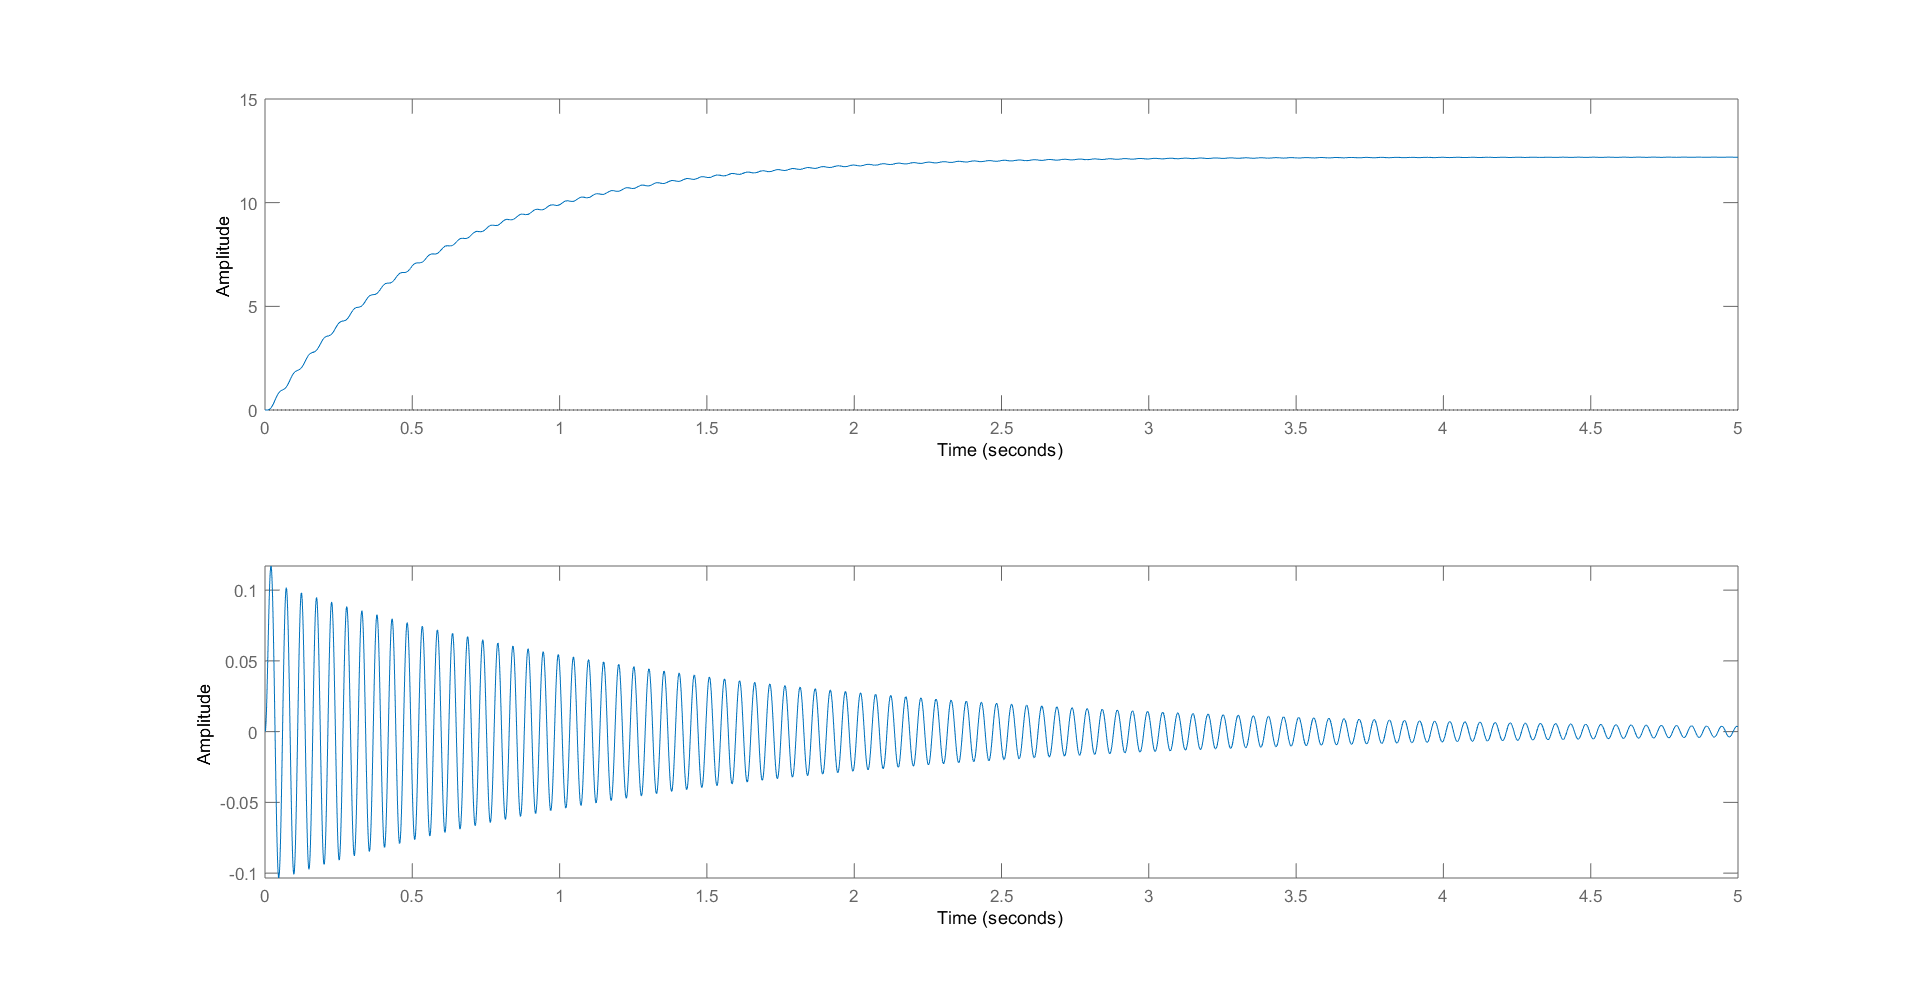
\includegraphics[width=0.7\textwidth]{h_mou}
	\captionof{figure}{Réponse impulsionnelle de l'arbre flexible et comparaison entre les deux systèmes.}
	\label{puissance}
\end{center}
On remarque que la réponse est très similaire à celle du système avec l'arbre rigide. 
De plus, les oscillations causées par le ressort torsionnel diminuent avec la stabilisation du système.



\section{Linéarisation}

\section{Conclusion}

La modélisation présentée dans ce rapport démontre que le système conçu pour
 l'asservissement de l'antenne remplis les requis d'EstampBeauce.








\begin{comment}
\begin{center}
	\centering
	\includegraphics[width=0.7\textwidth]{puissance}
	\captionof{figure}{Spectre de puissance d'une onde de 1kHz}
	\label{puissance}
\end{center}


\section{Filtres FIR}
\noindent\begin{minipage}{\textwidth} 
\begin{minipage}{0.5\textwidth}
  \centering
  \includegraphics[width=.75\linewidth]{ampFIR}
  \captionof{subfigure}{Amplitude}
  \label{FIR:ampFIR}
\end{minipage}%
\begin{minipage}{0.5\textwidth}
  \centering 
  \includegraphics[width=.75\linewidth]{phaseCute} 
  \captionof{subfigure}{Phase} 
  \label{FIR:phaseFIR} 
\end{minipage} 
\captionof{figure}{Filtre IIR} 
\label{FIR} 
\end{minipage}
\end{comment}

\end{document}













